\documentclass[12pt, dvipdfmx]{beamer}

\renewcommand{\kanjifamilydefault}{\gtdefault}
%%%%%%%%%%%  package  %%%%%%%%%%%
\usepackage{bxdpx-beamer}% dvipdfmxなので必要
\usepackage{pxjahyper}% 日本語で'しおり'したい

\usepackage{amssymb,amsmath,ascmac}
\usepackage{derivative}

\usepackage{multirow}
\usepackage{bm}

\graphicspath{{../fig/}}

\usepackage{animate}
\usepackage{tikz}
\usepackage{xparse}

%目次スライド
\AtBeginSection[]{
  \frame{\tableofcontents[currentsection]}
}
%アペンディックスのページ番号除去
\newcommand{\backupbegin}{
\newcounter{framenumberappendix}
\setcounter{framenumberappendix}{\value{framenumber}}
}
\newcommand{\backupend}{
\addtocounter{framenumberappendix}{-\value{framenumber}}
\addtocounter{framenumber}{\value{framenumberappendix}} 
}

%%%%%%%%%%%  theme  %%%%%%%%%%%
\usetheme{Copenhagen}
% \usetheme{Metropolis}
% \usetheme{CambridgeUS}
% \usetheme{Berlin}

%%%%%%%%%%%  inner theme  %%%%%%%%%%%
% \useinnertheme{default}

% %%%%%%%%%%%  outer theme  %%%%%%%%%%%
\useoutertheme{default}
% \useoutertheme{infolines}

%%%%%%%%%%%  color theme  %%%%%%%%%%%
%\usecolortheme{structure}

%%%%%%%%%%%  font theme  %%%%%%%%%%%
\usefonttheme{professionalfonts}
%\usefonttheme{default}

%%%%%%%%%%%  degree of transparency  %%%%%%%%%%%
%\setbeamercovered{transparent=30}

% \setbeamertemplate{items}[default]

%%%%%%%%%%%  numbering  %%%%%%%%%%%
% \setbeamertemplate{numbered}
\setbeamertemplate{navigation symbols}{}
\setbeamertemplate{footline}[frame number]


\title{粘着技術とタッキファイヤーの基礎\\と応用展開}
\subtitle{ ~ 第三章 粘着特性の理解に必要な物理について ~\\「高分子の振る舞いについて」}
\author[東亞合成 佐々木]{佐々木 裕\thanks{hiroshi\_sasaki@mail.toagosei.co.jp}}
\institute[東亞合成]{東亞合成株式会社}
\date{}

\begin{document}

%%%%%
% 1 P
%%%%%
\maketitle

\begin{frame} 
    \tableofcontents[]
\end{frame} 

\section{高分子とは?}
\begin{frame}
	\frametitle{高分子とは?}
		\begin{block}{高分子の性質}
			\begin{itemize}
				\item 「細くて」、「⻑くて」、「丸まった」
				\item グニャグニャ蠢くひものようなもの
			\end{itemize}
		\end{block}
		\centering
		\includegraphics[width=.8\textwidth]{polymer_image.jpg}
\end{frame}

\subsection{高分子は細くて長い}
\begin{frame}
	\frametitle{高分子は細くて長い}
	\centering
	\includegraphics[width=.8\textwidth]{polymer_model.png}
\end{frame}

\subsection{高分子は曲がって丸まる}
\begin{frame}
	\frametitle{高分子は曲がる}
	\centering
	\includegraphics[width=.8\textwidth]{polymer_model_2.png}
\end{frame}

\begin{frame}
	\frametitle{何故、高分子は曲がるのか?}
	回転異性体:トランスとゴーシュ
	\vspace{5mm}
	\centering
	\includegraphics[width=\textwidth]{butane.png}
\end{frame}

\begin{frame}
	\frametitle{高分子はクルクルと丸まる}
	\begin{itemize}
		\item 上の絵は、すべての結合がトランス状態
		\item ゴーシュが入ってくると曲がって、丸まる。
	\end{itemize}
	\centering
	\includegraphics[width=\textwidth]{PE.jpg}
\end{frame}

\begin{frame}
	\frametitle{高分子の大きさの見積もり}
	\centering
	\includegraphics[width=\textwidth]{polymer_R.png}
\end{frame}

\subsection{高分子は互いに入り組んでいる}
\begin{frame}
	\frametitle{高分子は互いに入り組んでいる}
	\centering
	\includegraphics[width=\textwidth]{polymer_penetrate.png}
\end{frame}

\begin{frame}
	\frametitle{高分子の絡み合いのイメージ}
	\begin{columns}[c, onlytextwidth]
		\column{.48\linewidth}
		\centering
		\includegraphics[width=\textwidth]{polymer_image2.png}

		多数の高分子鎖のイメージ
		\column{.48\linewidth}
		\centering
		\includegraphics[width=\textwidth]{karamiai.png}

		二本の高分子鎖の絡み合い
	\end{columns}
\end{frame}

\begin{frame}
	\frametitle{「高分子とは」のまとめ}
        \begin{boxnote}
            \vspace{-3mm}
            \begin{itemize}
                \item 高分子は細くて、長い
                    \begin{itemize}
                        \item 細くて長い紐のようなもの
                    \end{itemize} 
                \item 高分子は曲がる
                    \begin{itemize}
                        \item 二面角がゴーシュになると曲がる
                        \item 結果としてくるくると丸まる
                    \end{itemize} 
                \item 高分子は互いに入り組んでいる
                    \begin{itemize}
                        \item 丸まった球の中に他の鎖が多数入り込む
                        \item 非常に入り組んだ絡み合い
                    \end{itemize}
            \end{itemize}
        \end{boxnote}
\end{frame}

\section{高分子の振る舞いの温度依存性}
% \subsection{高分子の力学特性の温度依存性}
\begin{frame}
	\frametitle{高分子の力学特性の温度依存性}
			\begin{block}{教科書に示されている一般的な温度依存性}
				\begin{itemize}
					\item Tg 以下で、\textcolor{red}{ガラス状態⇔硬い固体}
					\item 転移領域を経て、\textcolor{green}{ゴム状態⇔柔らかい固体}
					\item より高温で、\textcolor{blue}{溶融・流動⇔液体}
				\end{itemize}
			\end{block}
				\vspace{3mm}
				\begin{center}
					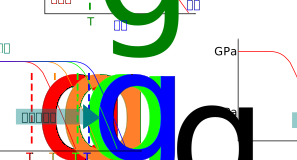
\includegraphics[width=.6\textwidth]{polymer_spectrum.png}
				\end{center}
\end{frame}

\subsection{高分子のガラス転移}
\begin{frame}
	\frametitle{高分子のガラス転移}
	\begin{itemize}
		\item MD シミュレーションで高分子のガラス転移を検討
		\item システムの体積変化を縦軸に
	\end{itemize}
	
	\vspace{-3mm}
	\begin{columns}[t, onlytextwidth]
		\column{.48\linewidth}
			\begin{block}{使用したポリマー}
				\begin{itemize}
					\item N=30
					\item 側鎖あり
				\end{itemize}
				% \vspace{-2mm}
				\centering
				\includegraphics[width=.7\textwidth]{N30_wSC1_single.png}
			\end{block}
		\column{.48\linewidth}
		\begin{center}
			\centering
			\includegraphics[width=.4\textwidth]{polymer_image2.png}

			\includegraphics[width=.8\textwidth]{N30_SC1_WA_K10.png}
		\end{center}
	\end{columns}
\end{frame}


\begin{frame}
	\frametitle{Tg 前後での運動性の変化}
		Tg 以上で運動性が大きく変化⇔粘性項が増大
		\begin{columns}[b, onlytextwidth]
			\column{.33\linewidth}
			\centering
			\textcolor{red}{Tg以下での\\凍結状態\\}
			\column{.33\linewidth}
			\centering
			\includegraphics[width=\textwidth]{N30_SC1_WA_K10.png}
			\column{.33\linewidth}
			\centering
			\textcolor{red}{Tg以上での\\自由な運動\\}
		\end{columns}
	
		\begin{columns}[c, onlytextwidth]
			\column{.48\linewidth}
			\centering
			\animategraphics[loop, width=\textwidth, autoplay]{20}{singlechain_lowTg/output_}{006}{027}

			\column{.48\linewidth}
			\centering
			\animategraphics[loop, width=\textwidth, autoplay]{20}{singlechain_highTg/output_}{006}{080}
		\end{columns}
\end{frame}

\begin{frame}
	\frametitle{低分子領域でのガラス転移の振る舞い}
		\begin{block}{MD シミュレーション}
			\begin{itemize}
				\item 連鎖延長でTg上昇し、数十個程度で収束
				\item Flory-Fox の式とよく一致
				\vspace{-1\baselineskip}
					\begin{align*}
						T_g = T_{g,\infty} - \dfrac{K}{Mn}
					\end{align*}
			\end{itemize}
			\vspace{-1\baselineskip}
		\begin{columns}[c, onlytextwidth]
			\column{.48\linewidth}
				\centering
				\includegraphics[width=.8\textwidth]{Tg_N_inv.png}
			\column{.48\linewidth}
				\centering
				\includegraphics[width=\textwidth]{polymer_spectrum_1.png}
		\end{columns}
	\end{block}
\end{frame}

\begin{frame}
	\frametitle{アクリル系材料のガラス転移温度の比較}
	アクリレートおよびメタクリレート類のガラス転移温度(Tg)を右図に示した。
		\begin{columns}[T, onlytextwidth]
			\column{.48\linewidth}
				\begin{itemize}
					\item 同一のアルコールからのエステルでは、メタクリルエステルの方が何十度も高温。
					\item 直鎖状の置換基が伸びれば、Tg は低下。
					\item バルキーな置換基で上昇。
				\end{itemize}
			\column{.48\linewidth}
				\vspace{-2mm}
				\includegraphics[width=.7\textwidth]{Tg.jpg}
				\vspace{-2mm}

				\tiny
			「機能性アクリレートの選び方・使い方 事例集」\\第2章第2節 技術情報協会
		\end{columns}
\end{frame}

\begin{frame}
	\frametitle{高分子混合物のガラス転移温度}
		\begin{block}{Fox の式}
			\begin{itemize}
				\item 高分子混合物のガラス転移温度を記述
				\item 前述の Flory-Fox の式からの拡張により提案
				\item 類似のポリマーの場合を想定していたが、相溶するものであれば適応可
				\item 溶媒や可塑剤と呼ばれる低分子でも適応可
				\begin{align*}
					&\dfrac{1}{T_g} = \dfrac{w_1}{T_{g,1}} + \dfrac{w_2}{T_{g,2}}\\
					&\text{$w_1, w_2$ はそれぞれの重量分率}
				\end{align*}
			\end{itemize}
		\end{block}
\end{frame}

\subsection{高分子のゴム状態}
\begin{frame}
	\frametitle{高分子のゴム状態}
			\begin{exampleblock}{ゴム状態の分子量依存性}
				\begin{itemize}
					\item 重合度が低いと、Tg 以上で直ちに流動
					\item 更なる高分子量化で、ゴム領域が高温化
					\item 互いの鎖が絡み合って束縛するため、ネットワークのように振る舞う。
				\end{itemize}
			\end{exampleblock}
			\vspace{3mm}
			\begin{columns}[c, onlytextwidth]
				\column{.48\linewidth}
					\centering
					\includegraphics[width=.9\textwidth]{polymer_spectrum_2.png}
				\column{.48\linewidth}
				\centering
				\includegraphics[width=.8\textwidth]{karamiai.png}
			\end{columns}
\end{frame}

\begin{frame}
	\frametitle{高分子のゴム状態での弾性率}
			% \begin{exampleblock}{ゴム状態の弾性率}
				\begin{itemize}
					\item 弾性率が一定となったゴム状態をラバープラトー
					\item この弾性的振る舞いはポリマー鎖のエントロピー由来
					\item このときの弾性率は\alert{ポリマー鎖の数密度 $\nu$ に比例}
					\item 溶媒や可塑剤と呼ばれる\alert{低分子の添加で弾性率低下}
				\end{itemize}
				\vspace{-.5\baselineskip}
					\begin{align*}
						G^{\prime} \propto \nu k_B T
					\end{align*}
				% \vspace{-1\baselineskip}
				\centering
						\includegraphics[width=.5\textwidth]{polymer_spectrum_rubber.png}
\end{frame}

\begin{frame}
	\frametitle{高分子のゴム状態での弾性率}
			% \begin{exampleblock}{ゴム状態の弾性率}
				\begin{itemize}
					\item ラバープラトーの弾性率は絡み合い状態に依存
					\item よく絡むポリマーの弾性率は高い(青線)
					\item 絡み合い点間の分子量 \alert{$M_E$ と弾性率は反比例}
				\end{itemize}
				\vspace{-.5\baselineskip}
					\begin{align*}
						G^{\prime} \propto \dfrac{1}{M_E}
					\end{align*}
				% \vspace{-1\baselineskip}
				\centering
						\includegraphics[width=.5\textwidth]{polymer_spectrum_rubber.png}
\end{frame}

\begin{frame}
	\frametitle{高分子を化学的に橋架すると}
			% \begin{exampleblock}{}
				% \begin{columns}[c, onlytextwidth]
				% 	\column{.58\linewidth}
					\begin{itemize}
						\item ガラス転移温度が上昇
						\begin{itemize}
							\item ポリマー鎖の運動性が低下してガラス化しやすくなる
						\end{itemize}
						\item それに伴い、ゴム領域での弾性率も上昇
						\begin{itemize}
							\item 架橋点間の鎖の数が増加し $\nu$ が増加
						\end{itemize}
                        \item \alert{流動化温度も上昇}
						% \begin{align*}
						% 	G^{\prime} \propto \nu k_B T
						% \end{align*}
					\end{itemize}
					% \column{.4\linewidth}
						\centering
						\includegraphics[width=.45\textwidth]{polymer_spectrum_3.png}
			% 	\end{columns}
			% \end{exampleblock}?
\end{frame}

\subsection{状態変化と緩和と損失弾性率}
\begin{frame}
	\frametitle{高分子の複数の緩和時間}
		\begin{columns}[c, onlytextwidth]
			\column{.5\linewidth}
			\begin{itemize}
				\item 実際の物質の内部は、\\大抵の場合、均一とは\\言えないことが多い。
				\item その結果として、マクロには複雑な緩和挙動を示す。
				\item \alert{仮想的}に、内部に\alert{複数の緩和時間}を考えよう。
				\item 右図のように\alert{モデル化}\\できる。
			\end{itemize}
			\column{.45\linewidth}
				\includegraphics[width=\textwidth]{relux_multi.png}
		\end{columns}
\end{frame}

\begin{frame}
	\frametitle{複数のマックスウェルモデル}
		\begin{block}{一般化マックスウェルモデル}
			\begin{itemize}
				\item \alert{それぞれの緩和時間に対応}するように、複数の\\マックスウェルモデルを想定し、
				\item すべてを、\alert{並列に連結}。
			\end{itemize}
		\end{block}
		\vspace{3mm}
		\centering
		\includegraphics[width=.8\textwidth]{relux_multi_2.png}
\end{frame}

\begin{frame}
    \frametitle{高分子での緩和}
			\begin{block}{たとえば、温度分散測定において}
				\begin{itemize}
					\item ガラス状態からの転移領域において
					\begin{itemize}
						\item 高分子鎖の\alert{運動性が大きく変化}
						\item 貯蔵弾性率が大きく低下
						\item 同時に\alert{損失弾性率が極大を示す}
					\end{itemize}
					\item 溶融流動においても同様な振る舞い
				\end{itemize}

				\vspace{2mm}
				\centering
				\includegraphics[width=.45\textwidth]{dynamic_ViscoElast_Temp.png}
			\end{block}
			
\end{frame}

\begin{frame}
    \frametitle{高分子での緩和}
			\begin{block}{周波数分散でも同様}
				\begin{itemize}
					\item ガラス状態からの転移領域において
					\begin{itemize}
						\item 高周波では動けなかった運動が動き出す
						% \item 貯蔵弾性率が大きく低下
						\item 同時に損失弾性率が極大を示す
					\end{itemize}
					\item \alert{温度分散を左右反転したような形に注意}
					\begin{itemize}
                        \item 低温は高周波(短時間)の振る舞いに相当
                    \end{itemize}
				\end{itemize}

				\vspace{2mm}
				\centering
				\includegraphics[width=.45\textwidth]{dynamic_ViscoElast_Freq.png}
			\end{block}
			
\end{frame}


\begin{frame}
	\frametitle{「高分子の振る舞いの温度依存性」のまとめ}
        \begin{boxnote}
            \vspace{-3mm}
            \begin{itemize}
                \item 高分子のガラス転移
                    \begin{itemize}
                        \item この温度で運動性が大きく変化
                        \item オリゴマー領域では分子量に依存して変化
                    \end{itemize} 
                \item 高分子のゴム状態
                    \begin{itemize}
                        \item 絡み合いが生じると流動できずにゴム状態
                        \item ラバープラトーの弾性率は鎖の数密度に比例
                    \end{itemize} 
                \item 状態変化と緩和と損失弾性率
                    \begin{itemize}
                        \item ガラス転移や流動において
                        \item 多様な緩和現象が生じ、損失弾性率が極大
                        \item 周波数分散でも同様な振る舞い
                    \end{itemize}
            \end{itemize}
        \end{boxnote}
\end{frame}

\section{高分子の相溶性}
\subsection{自由エネルギーによる系の記述}
\begin{frame}\frametitle{自由エネルギーによる系の記述}
	\begin{itemize}
		\item 系の\alert{有り様}を記述可能
		\item \alert{高分子は鎖が長いことに起因してエントロピー項の寄与が小さいため、丁寧な議論が必要}
		% \item その因子を考慮した Flory-Huggins 理論
	\end{itemize}

	\begin{block}{高分子特性を考慮した Flory-Huggins 理論}
		\begin{columns}[c, onlytextwidth]
			\column{.65\linewidth}
			\begin{itemize}
				\item ポリマーを同一体積のセグメントの連鎖で形成
				\item 格子状にポリマー鎖を配置
				\item 混合による体積変化はない
				\item 最近接格子点上のセグメント間にのみ相互作用エネルギー
			\end{itemize}
			\column{.3\linewidth}
					\centering
						\includegraphics[width=\textwidth]{FH_model.png}
				
		\end{columns}
	\end{block}
\end{frame}

\subsection{FH 理論による混合の自由エネルギー変化}
\begin{frame}\frametitle{FH 理論による混合の自由エネルギー変化}
	格子モデルでの混合自由エネルギー変化
	\vspace{-0.5\baselineskip}
	\begin{align*}
	f_{mix} &= \dfrac{F_{mix}}{\Omega k_B T} \notag \\
	&= \color{green}\left\{ \dfrac{\phi_A}{N_A} \log \phi_A 
	+ \dfrac{\phi_B}{N_B} \log \phi_B \right\} \color{black} 
	+ \color{blue}\chi \phi_A \phi_B \color{black}
	\end{align*}
	\color{green}第一項:エントロピー\color{black}、\color{blue}第二項:内部エネルギー\color{black}
	\begin{itemize}
	%\item 混合の自由エネルギー $F_{mix}$ $\Leftarrow$自由エネルギー密度
	%	\begin{itemize}
	%	\item 全格子点の数 $\Omega$ 、熱エネルギー $k_B T$ で規格化
	%	\end{itemize}
	\item  ポリマー $A$ と $B$ を混合(セグメント数が $N_A, N_B$)
	\item $\phi_A, \phi_B$ はそれぞれのポリマーの体積分率
	\item $\chi$ はセグメント同士の\color{red}相互作用パラメタ\color{black}
	\end{itemize}	
\end{frame}

\begin{frame}\frametitle{混合自由エネルギー曲線と相図}
    \begin{columns}[c, onlytextwidth]
        \column{.52\linewidth}
            \begin{block}{自由エネルギー曲線の例}
                \begin{itemize}
					\item 極小値一つ $\Rightarrow$ 一様混合
					\item 極小値が二つ $\Rightarrow$ 相分離
					\item 接点がバイノーダル組成
				\end{itemize}
                % \vspace{-0.5\baselineskip}
                \centering
					\includegraphics[width=.9\textwidth]{FE_tan_A10B20Chi0_2.png}
            \end{block}
        \column{.45\linewidth}
        \begin{exampleblock}{相図とは}
            \begin{itemize}
                \item 多数の $\chi$ パラメタ
                \item $\phi-\chi$ 平面上で
                \item 任意組成 $(\chi, \phi)$ の振る舞いを記述
            \end{itemize}
            % \vspace{-.5\baselineskip}
            \centering
                \includegraphics[width=.9\textwidth]{PD_6_600.png}
        \end{exampleblock}
    \end{columns}
\end{frame}

\subsection{相互作用パラメタ($\chi$)と相図}
\begin{frame}\frametitle{相互作用パラメタ($\chi$)と相図}
    \begin{block}{相図の読み方}
        \begin{itemize}
            \item スピノーダル線の内側ならば自発的に相分離
            \begin{itemize}
                \item 二相での体積分率はバイノーダル線上の値
                \item たとえば、$\chi=0.15$ の場合は図中の赤線
                \item スピノーダルの内側(太赤線)はどこでも同じふるまい
            \end{itemize}
            \item バイノーダル線の外側ならば一様溶解
        \end{itemize}
        \centering
		\includegraphics[width=.45\textwidth]{PD_6_600_4.png}
    \end{block}
\end{frame}

\begin{frame}
	\frametitle{「高分子の相溶性」のまとめ}
        \begin{boxnote}
            \vspace{-3mm}
            \begin{itemize}
                \item 自由エネルギーによる系の記述
                    \begin{itemize}
                        \item 高分子の混合においても自由エネルギー
                        \item 鎖の配置を考慮してエントロピーを議論
                    \end{itemize} 
                \item FH 理論による混合の自由エネルギー変化
                    \begin{itemize}
                        \item セグメント間相互作用を $\chi$ パラメタ
                        \item 鎖長に依存してエントロピー項が変化
                    \end{itemize} 
                \item 相互作用パラメタ($\chi$)と相図
                    \begin{itemize}
                        \item 相図は $\chi$ パラメタを縦軸、体積分率を横軸に、\\系の振る舞いを記述
                        \item 任意の組成の混合物の相分離の有無、および、\\それぞれの相での組成
                    \end{itemize}
            \end{itemize}
        \end{boxnote}
\end{frame}

\end{document}